\documentclass[../jarvis.tex]{subfiles}
\graphicspath{{\subfix{../images/}}}

\begin{document}
As it turns out, there's more to algebra than pure uninspiring symbol pushing. In this chapter we look at some structures and concepts in elementary algebra.

\begin{figure}[H]
    \centering
    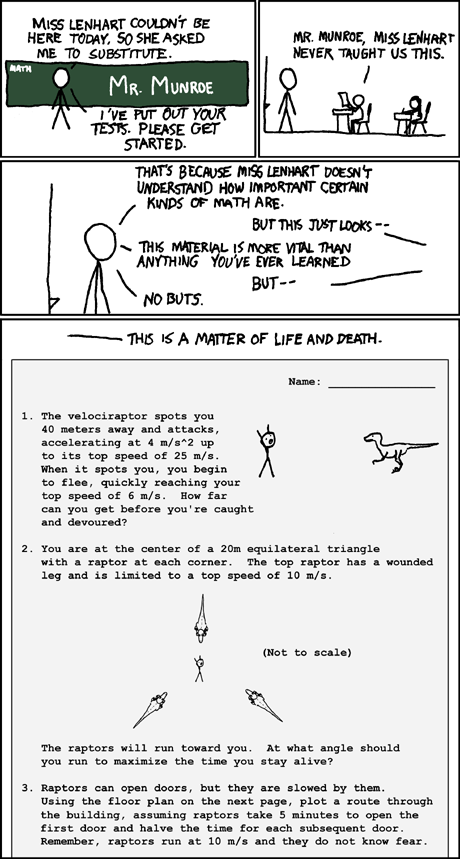
\includegraphics[scale=0.5]{xkcd_substitute.png}
    \caption{Comic from https://xkcd.wtf/135/}
\end{figure}

\subsection{Many Manipulations \ez}
\subsubsection{Factorising and Re-expressing}
Starting off easy, we will explore some funny-looking problems that solve themselves after some smart rearranging and rewriting.

\begin{example}[2013 SMO(J) P15]
    If $a=1.69$, $b=1.73$ and $c=0.48$, find the value of
    $$\frac{1}{a^2-ac-ab+bc}+\frac{2}{b^2-ab-bc+ac}+\frac{1}{c^2-ac-bc+ab}.$$
\end{example}
Of course, a good calculator can do this in seconds (although typing it in may take longer...), but what if you had to do this by hand? Substituting may not be smart...

However, we note that each of the denominators are suspiciously factorisable. For example,
$$a^2-ac-ab+bc=a(a-c)-b(a-c)=(a-b)(a-c).$$

\begin{proof}
    Hence,
\begin{align*}
    & \frac{1}{a^2-ac-ab+bc}+\frac{1}{b^2-ab-bc+ac}+\frac{1}{c^2-ac-bc+ab}\\
    &=\frac{1}{(a-b)(a-c)}+\frac{2}{(b-c)(b-a)}+\frac{1}{(c-b)(c-a)} \\
    &=\frac{(b-c)-2(a-c)+(a-b)}{(a-b)(a-c)(b-c)} \\
    &=-\frac{1}{(a-b)(b-c)} = -\frac{1}{(-0.04)(1.25)} = \boxed{20}
\end{align*}
\end{proof}


\begin{example}[2013 SMO(J) P32]
    If $a$ and $b$ are positive integers such that $a^2+2ab-3b^2-41=0$, find $a^2+b^2$.
\end{example}
The constant "$41$" seems irrelevant to the equation at this point, except that it's a prime number (this may be important!). For now, let us write the equation as $a^2+2ab-3b^2=41$.

\begin{proof}
    Notice that the coefficients of the LHS sum to $(1+2-3=)0$(!), so this tells us that we should factorise:
$$a^2+2ab-3b^2=a^2-ab+3ab-3b^2=a(a-b)+3b(a-b)=(a+3b)(a-b)=41.$$

Now, it becomes apparent why $41$ was chosen: because it is a prime number, and $a,b$ are integers, $a+3b$ and $a-b$ are each either $1$ or $41$. Moreover, $a+3b \geq a-b$ so we have
$$
\begin{cases}
    a+3b&=41 \\
    a-b&=1
\end{cases} \implies a=11, b=10.
$$
Thus, $a^2+b^2=11^2+10^2=\boxed{221}$.
\end{proof}


\begin{example}[2017 SMO(J) P20]
    Let $a$, $b$ and $c$ be positive integers such that
    $$a^2+bc=257\quad\text{and}\quad ab+bc=101.$$

    Find the value of $a$, $b$ and $c$.
\end{example}
\begin{proof}
    Armed with the idea from the previous problem, we see again that $101$ is a prime number, so $b(a+c)=101$. Moreover, $b+c\geq a$ so that $b=1$ and $a+c=101$. Thus, $$a^2+bc=a^2+c=a^2+(101-a)=257 \implies a(a-1)=156.$$

    With some guess and check (since $a$ is a positive integer), $a=13$, $b=1$ and $c=88$.
\end{proof}


\begin{example}[2016 SMO(J) P24]
    If $\frac{a}{2b}=\frac{2b}{3c}=\frac{3c}{8a}$, find the value of $\frac{ac+cb}{cb-ba}.$
\end{example}
The given condition tells us that $a$, $b$ and $c$ are all connected, so we should express $a$ and $b$ in terms of $c$.

\begin{proof}
    Let $\frac{a}{2b}=\frac{2b}{3c}=\frac{3c}{8a}=k$ for some real $k$. We have
$$ 
\begin{cases}
    a=2kb \\
    2b=3kc \\
    3c=8ka
\end{cases}
\implies
\begin{cases}
    a=3k^2c \\
    2b=8k^2a \\
\end{cases}
\implies
\begin{cases}
    a=24k^5c \\
    b=12k^4c    
\end{cases} 
.$$
By the given condition, we have $\frac{2b}{3c}=\frac{24k^4c}{3c}=8k^4=k \implies 8k^3=1 \implies k=\frac{1}{2}$, $k^5=\frac{1}{32}$

Hence,
\begin{align*}
    \frac{ac+cb}{cb-ba}
    &= \frac{24k^5c^2+12k^4c^2}{12k^4c^2-288k^9c^2} \\
    &= \frac{2k+1}{1-24k^5} \\
    &= \frac{2\cdot\frac{1}{2}+1}{1-24\cdot\frac{1}{32}} = \boxed{8}
\end{align*}
\end{proof}

\subsubsection{Homogenisation}
For our first concept of the handout, we introduce the trick of counting degrees, or \textit{homogenisation}. We only illustrate as such with a simple problem, and further applications of this idea will follow in a later.

\begin{proposition}[Counting degrees]
    We say that an expression or equation is \textit{homogenous} (or homogenised) if there is no loose constant terms remaining. For example, $x^3+2022x^2y+2021$ is non-homogenous because of the constant $2021$, while $x^3+2022xy^3+xy$ is homogenous because there is no loose constant. 

    We \textit{want} to work with homogenous expressions because degrees cancel nicely, and expressions are usually neat. 
\end{proposition}
\begin{example}
    If $x$ and $y$ are real numbers such that $x+y=2$ and that
    $$\frac{(1-x)^2}{x}+\frac{(1-y)^2}{y}=-4,$$
    find the value of $xy$.
\end{example}

Consider the term $\frac{(1-x)^2}{x}$. The numerator is a quadratic (degree $2$) while the denominator is linear (degree $1$), so we say that this term is of degree $1$. The term $\frac{(1-y)^2}{y}$ is also similarly of degree $1$, and so the LHS is of degree $1$. 

On the other hand, the RHS is a constant (degree $0$), which makes the equation \textit{non-homogenous}. Fortunately, we are given that $x+y=2$. 

\begin{proof}
    We begin by writing
$$\frac{(1-x)^2}{x}+\frac{(1-y)^2}{y}=-2(x+y).$$ Now, our equation is homogenous, and as we shall see, this equation now resolves itself very cleanly. Clearing denominators (since $x,y \neq 0$), we have
\begin{align*}
    \frac{(1-x)^2}{x}+\frac{(1-y)^2}{y}=-2(x+y) &\implies x(1-y)^2+y(1-x)^2=-2xy(x+y) \\
    &\implies (xy^2-2xy+x)+(x^2y-2xy+y)=-2x^2y-2xy^2 \\
    &\implies 3x^2y+3xy^2-4xy+(x+y)=0 \\
    &\implies 3xy(x+y)-4xy+(x+y)=0 \\
    &\implies 2xy+2=0 \implies xy=\boxed{-1}
\end{align*}
\end{proof}

\subsubsection{Substitutions and Identities}
Sometimes scary expressions are just expanded versions of simpler expressions! A smart substitution will help simplify things nicely. Certainly, knowing some basic identities will help reduce the problem. Here, we list the necessary few.

\begin{proposition}[Basic Identities]
    These identities can also be found in school textbooks, and familiarity is assumed.
    \begin{enumerate}
        \item $a^2-b^2=(a-b)(a+b)$
        \item $a^2\pm 2ab+b^2=(a\pm b)^2$
        \item $a^3\pm b^3=(a\pm b)(a^2\mp ab+b^2)$
        \item $a^3+3a^2b+3ab^2+b^3=(a+b)^3$
        \item $a^3-3a^2b+3ab^2-b^3=(a-b)^3$
    \end{enumerate}
\end{proposition}

To start off, we showcase an application of a nifty substitution, without which, the problem may be untractable to the unsuspecting student.
\begin{example}[2013 SMO(J) P11]
    Find the value of $\sqrt{9999^2+19999}.$
\end{example}
Certainly, we are not expected to multiply out and then take the square root of this monstrous expression! However, we do note that the choice of $9999$ is completely arbitrary, so it may be wise to make a substitution for $9999$ and express $19999$ in terms of $a$.

\begin{proof}
    Let $a=9999$, then $19999=2\cdot 9999+1=2a+1$. Aha! We now know
\begin{align*}
    \sqrt{9999^2+19999}&=\sqrt{a^2+(2a+1)} \\
    &=\sqrt{(a+1)^2}=a+1 \\
    &=\boxed{10000}.
\end{align*}
How nice is that!
\end{proof}

\begin{example}[2014 SMO(J) P16]
    Let $m$ and $n$ be positive real numbers satisfying the equation
    $$m+4\sqrt{mn}-2\sqrt{m}-4\sqrt{n}+4n=3.$$
    Find the value of $$\frac{\sqrt{m}+2\sqrt{n}+2014}{4-\sqrt{m}-2\sqrt{n}}.$$
\end{example}
The required value is just as grizzly as the given equation. To start, we should be somewhat suspicious of the term $4\sqrt{mn}$: this is a term of degree $1$, since $\sqrt{m}$ and $\sqrt{n}$ both have degree $\frac{1}{2}$. Yet, it's mixed in an expression containing terms of degree $\frac{1}{2}$ like $2\sqrt{m}$ and $4\sqrt{n}$, as well as degree $1$ terms like $m$ and $4n$.

This strongly suggests the substitutions $x=\sqrt{m}, y=\sqrt{n}$, so we want the value of 
$$\frac{\sqrt{m}+2\sqrt{n}+2014}{4-\sqrt{m}-2\sqrt{n}}=\frac{x+2y+2014}{4-(x+2y)}.$$

The given equation gives $$x^2+4xy-2x-4y+4y^2=3. \implies (x+2y)^2-2(x+2y)=3 \implies (x+2y)(x+2y-2)=3.$$ Setting $z=x+2y$, $z(z-2)=3 \implies z^2-2z-3=0 \implies z=3$ only since $z=x+2y>0$. 

Hence, the required value is \boxed{4}.

\begin{example}[2015 SMO(J) P21]
    Find the value of $$\sqrt{(98\cdot 100+2)(100\cdot 102+2)+(100\cdot 2)^2}.$$
\end{example}
Once again, this is a monstrous expression, but fortunately the individual parts in the expression are broken down slightly for us. For now, let us focus on the term $98\cdot 100+2$. 

It may be tempting to simply substitute $a=98$ (or $a=100$), but the expression $a(a+2)+2=a^2+2a+2$ is cumbersome to work with. Perhaps we should compromise and let $a=99$ instead!

Then, $98\cdot 100+2= (a-1)(a+1)+2=a^2+1=99^2+1$, and similarly, $100\cdot 102+2 = 101^2+1$. The desired expression is now
$\sqrt{(99^2+1)(101^2+1)+(100\cdot 2)^2}$, and it is apparent why $100\cdot 2$ was written instead of $200$. Letting $b=100$, we have
\begin{align*}
    \sqrt{(99^2+1)(101^2+1)+(100\cdot 2)^2}&=\sqrt{((b-1)^2+1)((b+1)^2+1)+4b^2}\\
    &=\sqrt{(b^2-2b+2)(b^2+2b+2)+4b^2} \\
    &=\sqrt{((b^2+2)-2b)((b^2+2)+2b)+4b^2} \\
    &=\sqrt{(b^2+2)^2-(2b)^2+4b^2} \\
    &= b^2+2=\boxed{10002}
\end{align*}

\begin{example}[2018 AMC10 A/10]
    Suppose that real number $x$ satisfies $$\sqrt{49-x^2}-\sqrt{25-x^2}=3.$$
    Find the value of $\sqrt{49-x^2}+\sqrt{25-x^2}$.
\end{example}
The given equation is an equation in terms of $x^2$, so it would be instinctive to substitute $y=x^2$ and then squaring both sides and rearranging:
\begin{align*}
    \sqrt{49-y}-\sqrt{25-y}=3 &\implies 74-2y-2\sqrt{(49-y)(25-y)}=9 \\
    &\implies 2\sqrt{(49-y)(25-y)}=65-2y\\
    &\implies 4(49-y)(25-y)=(65-2y)^2 \\
    &\implies 4(y^2-74y+1225)=4y^2-260y+4225 \\
    &\implies -36y+675=0 \implies y=\frac{75}{4},
\end{align*}
whence the required value is 
$$\sqrt{49-x^2}+\sqrt{25-x^2}=\sqrt{49-y}+\sqrt{25-y}=\sqrt{\frac{121}{4}}+\sqrt{\frac{25}{4}}=\boxed{8}.$$

This method feels slightly disingenous though, why would the problem seek such a specific quantity? On a closer look, we notice that the given expression and the required expression are very similar. In particular, they differ only in their signs!

If we let $a=\sqrt{49-x^2}$ and $b=\sqrt{25-x^2}$, then $a-b=3$ and we seek the value of $a+b$.

This reminds us of the \textit{difference of squares} identity, and we finish the problem succinctly:
\begin{proof}
    $$(a-b)(a+b)=a^2-b^2=(49-x^2)-(25-x^2)=24.$$
On the other hand, 
$$3(a+b)=24 \implies \sqrt{49-x^2}+\sqrt{25-x^2}=a+b=\frac{24}{3}=\boxed{8}.$$
\end{proof} 

For our ending problem, we showcase the idea of \textit{rationalisation} for cube roots. Indeed, at the heart of rationalising surds, we rely on the difference of squares. As it turns out, this also works for cube roots! 
\begin{example}[2013 AIME II/5]
    Find the real root of the equation $8x^3-3x^2-3x-1=0$ in the form 
    $$x=\frac{\cbrt{a}+\cbrt{b}+1}{c},$$
    where $a,b,c$ are positive integers.
\end{example}
Firstly, the coefficients $3, 3, 1$ seem vaguely familiar. In fact, $(x+1)^3=x^3+3x^2+3x+1$. Thus, we write
$$8x^3-3x^2-3x-1=9x^3-(x^3+3x^2+3x+1)=9x^3-(x+1)^3,$$
whence $9x^3=(x+1)^3$.

Solving for $x$, we have $$x=\frac{1}{\cbrt{9}-1}.$$ We make the substitution $a=\cbrt{9}$, and so $a^3=9$. The cube root suggests that the difference of cubes formula may be useful. Indeed, $$(a-1)(a^2+a+1)=a^3-1,$$ and so
\begin{align*}
    x&=\frac{1}{\cbrt{9}-1}=\frac{1}{a-1} \\
    &=\frac{1}{a-1}\cdot \frac{a^2+a+1}{a^2+a+1}=\frac{a^2+a+1}{a^3-1} \\
    &=\frac{\cbrt{81}+\cbrt{9}+1}{8}.
\end{align*}

\subsection{Some Solving}
Many questions will demand you to "find all X satisfying condition Y", the keyword being \textbf{find all}. These problems come in solving equations, functional equations, inequalities, etc. This implies that there are two parts to the problem: 
\begin{enumerate}
    \item Find the solutions and show that no other solutions exist.
    \item Prove that your solutions satisfy the condition (this is part of the problem!).
\end{enumerate}
It will be more instructive for us to work through a problem.

\begin{example}[2021 SMO(O) P10]
Find all real roots to the equation
$$\sqrt[9]{x^7+30x^5}=\sqrt[7]{x^9-30x^5}.$$
\end{example}
As a first scout, we see that $x=0$ is a solution. Moreover, if $x=k$ is a solution, then so is $x=-k$, so we may consider only $x > 0$.
\begin{proof}
Let $a=\sqrt[9]{x^7+30x^5}$, $b=\sqrt[7]{x^9-30x^5}$ so that
$$\begin{cases}
    a-b=0 \\
    a^9+b^7=x^{16}
\end{cases}
\implies
a^{16}=x^{16} \implies a=\pm x.$$

If $a=x$, then $a^9=a^7+30a^5.$ 

Aha! This gives our first solution $a=0$, corresponding to $x=0$. In what follows, we assume $x\neq 0 \implies a\neq 0$.

Thus, $a^4=a^2+30 \implies (a^2-6)(a^2-5)=0 \implies a=\pm \sqrt{5}, a=\pm \sqrt{6}$.

Now, are all of these valid solutions? We should verify so. Suppose $a=x=\sqrt{5}$ (since we have $x>0$), then 
$$a^9=625\sqrt{5}=125\sqrt{5}+750\sqrt{5}=875\sqrt{5},$$ which is a contradiction. Thus $x\neq \sqrt{5}$.
\begin{remark}
Notice the use of proof by contradiction here! We assumed that $x=\sqrt{5}$ is a solution, and then derived the absurd statement that $625\sqrt{5}=875\sqrt{5}$.
\end{remark}
Similarly, suppose $a=x=\sqrt{6}$, then $a^9=1296\sqrt{6}=216\sqrt{6}+1080\sqrt{6}$, which is consistent. Hence, $a=\sqrt{6}$ is the solution we're after. Having exhausted all cases, and verified that our solution was correct, we can now confidently say that the only solutions to the original equation are $$\boxed{\text{$x=0$, $\sqrt{6}$ and $-\sqrt{6}$}}.$$
\end{proof}

Before we go further, we note that sometimes a polynomial is  hard to factorise, especially if it has high degrees or have large coefficients. The Rational Root Theorem is extremely useful to help us discover any potential linear factors and rational roots.
\begin{proposition}[Rational Root Theorem]
For a polynomial $P(x)=a_nx^n+a_{n-1}x^{n-1}+\cdots+a_1x+a_0$ with real coefficients $\{a_n\}=0$, if $P(x)$ \textit{has a rational root} $x=\frac{p}{q}$ where $\gcd(p,q)=1$, then
\begin{itemize}
    \item $p$ is an integer factor of the constant term $a_0$, and
    \item $q$ is an integer factor of the leading coefficient $a_n$.
\end{itemize}
It is important to point out that this \textbf{does not} guarantee that $P(x)$ has a rational root. It merely proposes that there are candidates.
\end{proposition}

Let's see it in action:
\begin{example}[2021 SMO(S) P22]
Find all real solutions $(x,y)$ to the system
\begin{align}
    x^3+y^3+y^2&=0 \label{13-sys-1} \\
    x^2+x^2y+xy^2&=0 \label{13-sys-2}
\end{align}
\end{example}
This is a tough system: both equations are cubic in nature. As an initial scout, it's wise to guess a few solutions: since $x$ is the "lone variable" in equation 2, letting $x=0$ gives $y=0, -1$. We also see that $x=y$ is another solution. In particular, if $x=y$, we have $$2y^3+y^2=0 \implies y=0, -\frac{1}{2}.$$

Thus, we immediately have the solutions $(0,0)$, $(0,-1)$ and $(0, -\frac{1}{2})$, and we know these are (likely) all the solutions because the system has degree 3 (we still need to verify whether there are other nontrivial classes of solution).

\begin{proof}
    To start, we see that \eqref{13-sys-2} is a quadratic in $x$, so $x^2(1+y)+xy^2=0.$ If $x=0$, then we get the three solutions as above. If $y=-1$ in \eqref{13-sys-1}, we have $x=0$, as above. So, suppose $x\neq 0, y\neq -1$, then
$$x(1+y)+y^2=0 \implies x=-\frac{y^2}{1+y}.$$

Putting this into \eqref{13-sys-1}, 
$$-\frac{y^6}{(1+y)^3}+y^2(1+y)=0 \implies \frac{-y^6+y^2(1+y)^3}{(1+y)^4}=0 \implies 4y^3+6y^2+4y+1=0.$$

To factorise this, we use the rational root theorem. The potential roots are thus $y=\pm 1, \pm \frac{1}{2}, \pm\frac{1}{4}$, and from our scouting, we know $y=-\frac{1}{2}$ is a root. Thus,
$$4y^3+6y^2+4y+1=0=(2y+1)(2y^2+2y+1)=0,$$
where the quadratic factor has no real solutions to it. Thus, having exhausted all cases, we have recovered the solutions
$$\boxed{(x,y)=(0,0), (0,-1), (0,-\frac{1}{2})}.$$
\end{proof}

This next problem showcases the mixing of algebra and a string of divisibility arguments. Keep an eye out for these, especially if we are solving over the integers!
\begin{example}[2018 SMO(O) P9]
    Let $p(x)=x^3+ax^2+bx+c$ be a polynomial where $a,b,c$ are distinct non-zero integers. Suppose $p(a)=a^3$ and $p(b)=b^3$. Find $p(13)$.
\end{example}
Hmm, somehow we are apparently able to determine the cubic with only 2 given points. Perhaps the distinct and integer condition will come into play somehow. (For the astute reader, this matches the four degrees of restriction we need to determine a cubic - just as we need four points to determine a cubic as well.)
\begin{proof}
    Given $p(a)=a^3$ and $p(b)=b^3$, we have 
    \begin{align*}
        a^3+ab+c&=0\\
        (a+1)b^2+c&=0
    \end{align*}
    Eliminating $c$,
    we have $(a+1)b^2-ab-a^3=0$, which is a quadratic in $b$.
    
    Using the quadratic formula,
    \begin{align*}
        b&=\frac{a\pm \sqrt{a^2+4a^3(a+1)}}{2(a+1)}\\
        &=\frac{a\pm a\sqrt{4a^2+4a+1}}{2(a+1)}=\frac{a\pm a(2a+1)}{2(a+1)} \\
        &=a \quad \textbf{or} \quad -\frac{a^2}{a+1}
    \end{align*}
    Since $a,b$ are distinct, we must have $b=-\frac{a^2}{a+1}.$
    Moreover, since $b$ is an integer, 
    $$b=-\frac{a^2}{a+1}=-(a-1)-\frac{1}{a+1}$$
    is also an integer. This means $a+1|1 \implies a+1=\pm 1$, giving $a=-2$ only. Thereafter, $b=4$ and $c=16$ follows easily, whence the answer is 
    $$p(13)=13^3-2\cdot 13^2+4\cdot 13+16=\boxed{1927}$$
\end{proof}

While more involved in nature, this next problem showcases just how powerful a string of divisibility arguments can be.
\begin{example}[USAMO 2015 P1, JMO P2]
Solve in integers the equation
$$x^2+xy+y^2=\left(\frac{x+y}{3}+1\right)^3.$$
\end{example}
To start off, we know LHS is an integer and so RHS must also be an integer. This means $\frac{x+y}{3}$ is also an integer, so we are motivated to write $x+y=3k$ for some integer $k$.

On the other hand, LHS contains a pesky $xy$ term. Here comes the \textit{trick}: to kill off this nasty term, we rely on the symmetry of $x$ and $y$. 
\begin{proof}
    Consider $a=x+y, b=x-y$:
    $$xy= \frac{(a+b)(a-b)}{4} \quad\text{and}\quad x^2+y^2= \frac{(a+b)^2+(a-b)^2}{4}$$
and the equation becomes
$$\frac{1}{4}\left((a+b)^2+(a+b)(a-b)+(a-b)^2\right)=\left(\frac{a}{3}+1\right)^3 \implies 3a^2+b^2=4\left(\frac{a}{3}+1\right)^3.$$
Letting $a=3k$, $27k^2+b^2=4(k+1)^3 \implies b^2=4k^3-15k^2+12k+4$.
At this point, surely the cubic must factor. Indeed, we miraculously see
$$b^2=(k-2)^2(4k+1) \implies 4k+1=m^2,$$
for odd $m$ (see the problem above for a similar reasoning).

Now, we are done, since by back-substituting, we have:
$$a=3k=\frac{3}{4}(m^2-1), \quad b^2=(k-2)^2(4k+1)=\left(\frac{m^2-9}{4}\right)^2m^2 \implies b=\pm \frac{m^3-9m}{4}.$$
Hence,
$$x=\frac{1}{8}\left(3(m^2-1)\pm(m^3-9m)\right)\quad\text{and}\quad y=\frac{1}{8}\left(3(m^2-1)\mp(m^3-9m)\right).$$

Is that all? Not quite! Don't forget that we are told to solve the given equation over the integers, so we should show also that our solutions are indeed all integers. Fortunately, since $m$ is odd, we may let $m=2n+1$ so that
$$\boxed{x=n^3+3n^2-1\quad\text{and}\quad y=-n^3+3n+1},$$
and permutations (note that the equation is symmetric in $x$ and $y$!).
\end{proof}

Finally, we end off with this problem: still on divisibility arguments, but this time it's on the unique prime factorisations!
\begin{example}[2021 H3 Math P1 Q4]
Let $a,b,c,d$ be positive integers such that
\begin{equation}\label{5.3-det}
    (ad-bc)^2=(a+b)(c+d)
\end{equation}
Show that there exists coprime positive $x,y$ and a positive integer $z$ such that
$$a+b=x^2z, c+d=y^2z.$$
\end{example}
Here, we say that two integers $r,s$ are \textbf{coprime} (or \textbf{relatively prime}) \textit{if and only if} $\gcd(r,s)=1$, meaning that their greatest common factor is $1$. The readers more familiar with number theory will quickly recall that the problem implies that $\gcd(a+b, c+d)=z$.

Indeed, we may claim as such, since the problem only asks of us to prove the existence of \textit{a} positive integer $z$. We begin by defining $z=\gcd(a+b, c+d)$, whence $a+b=mz$, $c+d=nz$ for some coprime $m, n$. Our goal is now to show that $m$ and $n$ are both perfect squares.

From \eqref{5.3-det}, $(ad-bc)^2=mnz^2$, so $mn$ is a perfect square. Now, consider the prime decompositions:
    $$m = \prod {p_i}^{e_i}, \;n = \prod {q_j}^{f_j}$$
Since $m$ and $n$ are coprime, no $p_i$ and $q_j$ are equal.
Moreover,
$$mn = {p_1}^{e_1}\cdot{p_2}^{e_2}\cdots{q_1}^{f_1}\cdot{q_2}^{f_2}\cdots.$$
Since $mn$ is a perfect square, all $e_i$ and $f_j$ are even, which implies that $m$ and $n$ are both perfect squares.

Now, we may write $m=x^2$, $n=y^2$ for some coprime $x,y$ since $m, n$ are coprime. Plugging this back into our original definition, we have $a+b=x^2z, c+d=y^2z$, as required.
\begin{example}[cont.]
Find a quadratic equation that $\frac{y}{x}$ satisfies, and hence prove that $4ac+1$ is a perfect square.
\end{example}
We have
$$\frac{y^2}{x^2}=\frac{c+d}{a+b}.$$
Square-rooting this term is slightly obstructive, so we should find another way to express $\frac{y}{x}$. Since we have not used $\eqref{5.3-det}$, this might be the time. Dividing across by $(a+b)^2$ (since it is non-zero), we have
$$\frac{(ad-bc)^2}{(a+b)^2}=\frac{c+d}{a+b}=\frac{y^2}{x^2} \implies \frac{ad-bc}{a+b}=\frac{y}{x}$$
since $\frac{y}{x}$ is positive.

Our quadratic is
\begin{align*}
   &\frac{py^2}{x^2}+\frac{qy}{x}+r=\frac{p(c+d)}{a+b}+\frac{q(ad-bc)}{a+b}+r=0 \\
   \Longleftrightarrow &p(c+d)+q(ad-bc)+r(a+b)=0
\end{align*}

This means we should make a choice for $p, q$ and $r$. Let us investigate this observation: if we choose $p=a, r=-c$,
\begin{align*}
    a(c+d)+q(ad-bc)-c(a+b)&=ac+ad+q(ad-bc)-ac-bc\\
    &=ad+q(ad-bc)-bc=0,
\end{align*}
almost as if it's forcing $q=-1$!
Thus, a possible quadratic equation is $au^2-u-c=0$ with $u=\frac{y}{x}$.

Now, if $x$ is a rational root, then we realise that $\Delta$ needs to be a rational square, that is the square of a rational number, and that this condition also implies that $x$ is a rational root. We say that this bi-directional relationship is a \textbf{necessary and sufficient} condition. In this problem, $\frac{y}{x}$ is a rational root to our quadratic, so $4ac+1$ is a rational square. However, $4ac+1$ is also a positive integer, and so it must be a perfect square!

As again, proofs should be written in the forwards direction, and we present so succinctly.
\begin{proof}
I claim that the quadratic equation is $au^2-u-c=0$ if $ad-bc > 0$ and $au^2+u-c=0$ if $ad-bc < 0$.

We have $$\frac{y^2}{x^2}=\frac{c+d}{a+b} \quad\text{and}\quad \frac{y}{x}=\frac{ad-bc}{a+b},$$
Thus, $$a\left(\frac{c+d}{a+b}\right)-\left(\frac{ad-bc}{a+b}\right)-c=\frac{a(c+d)-(ad-bc)-c(a+b)}{a+b}=0.$$

The discriminant is $\Delta=4ac+1$. Since $\frac{y}{x}$ is a rational root, $\Delta$ is a rational square. Moreover, $4ac+1$ is a positive integer, and so it is a perfect square.
\end{proof}
\begin{moral}
The main challenge was discovering the quadratic equation, but we are motivated by the term $4ac+1$, which reminded us of the quadratic discriminant. Finally, the treatment of $\Delta$ required us to recall the definition of the discriminant and to argue that it must be a rational square, which implied that it is also a perfect square given that $a,b,c,d$ are all integers.
\end{moral}
\end{document}